\documentclass[11pt, a4paper, twoside]{article}
\usepackage{graphicx}
\usepackage{amsmath}
\usepackage[margin=0.8in]{geometry}
\usepackage{listings}
\usepackage{float}
\usepackage{fancyhdr}
\usepackage{indentfirst}
\usepackage[inline]{enumitem}
\usepackage{tabularx}
\usepackage{xcolor}
\usepackage{array}
\usepackage{minted}
\usemintedstyle{vs}
\usepackage[belowskip=0pt,aboveskip=0pt,font=small,labelfont=small]{caption}
\captionsetup{width=\linewidth}
\setlength\intextsep{0pt}
\graphicspath{{Plots/}}
\setlist[itemize]{noitemsep, topsep=0pt}
\fancyhead[RO,LE]{EE2703: Assignment 6}
\fancyhead[LO,RE]{Akilesh Kannan}
\cfoot{\thepage}

\title{EE2703: Assignment 6}
\author{Akilesh Kannan (EE18B122)}
\date{\today}

\pagestyle{fancy}

\begin{document}
\maketitle

\section{Introduction}
    We analyse LTI systems in continuous time using Laplace transforms to find the output of the system to a given input with the help of a python library, namely \texttt{scipy.signal} toolbox.

\section{Time Response of Spring Oscillator}
    Our goal is to find the response of a spring oscillator, governed by the equation:
    \begin{equation*}
        \ddot{x} + 2.25x = f(t)
    \end{equation*}

    where,
    \begin{gather*}
        x(t) = \text{Displacement of spring}\\
        f(t) = \text{Force applied on the spring}
    \end{gather*}

    We consider the case that the force applied on the spring is given by:
    \begin{equation*}
        f(t) = e^{-at}cos(\omega t)u(t)
    \end{equation*}

    We shall do a case by case analysis for the following values of a and $\omega$:

    \begin{center}
        \begin{tabularx}{0.4\textwidth} {
            | >{\centering\arraybackslash}X
            || >{\centering\arraybackslash}X | }
             \hline
             a ($sec^{-1}$)&$\omega$ ($rad\ sec^{-1}$)  \\
             \hline
             \hline
             0.5&1.5  \\
             \hline
             0.05&1.5 \\
             \hline
             0.05&1.4 \\
             \hline
             0.05&1.45 \\
             \hline
             0.05&1.5 \\
             \hline
             0.05&1.55 \\
             \hline
             0.05&1.6 \\
             \hline
        \end{tabularx}
    \end{center}
    \subsection{Power of Laplace transforms}
        The Laplace transform of $f(t) = e^{-at}cos(\omega t)u(t)$ is given as:
        \begin{equation*}
            \mathcal{L}\{f(t)\} = \frac{s+a}{(s+a)^2 + \omega^2}
        \end{equation*}

        From the property of Laplace transforms, we know:
        \begin{gather*}
            x(t) \longleftrightarrow \mathcal{X}(s)\\
            \implies \dot{x}(t) \longleftrightarrow \ s\mathcal{X}(s) - x(0^-)\\
            \implies \ddot{x}(t) \longleftrightarrow \ s^2\mathcal{X}(s) - sx(0^-)-\dot{x}(0^-)
        \end{gather*}

        From the above equations, we get, for $a = 0.5$ and $\omega = 1.5$:
        \begin{equation*}
            \mathcal{F}(s) = \mathcal{L}\{f(t)\} = \frac{s+0.5}{(s+0.5)^2+2.25}
        \end{equation*}

        So, the equation of the spring oscillator can be written as:
        \begin{equation*}
            s^2\mathcal{X}(s) - sx(0^-)-\dot{x}(0^-) + 2.25\mathcal{X}(s) = \frac{s+0.5}{(s+0.5)^2+2.25}
        \end{equation*}

        Given that the ICs $x(0)$ and $\dot{x}(0)$ are 0, we get:
        \begin{equation*}
            s^2\mathcal{X}(s) + 2.25\mathcal{X}(s) = \frac{s+0.5}{(s+0.5)^2+2.25}
        \end{equation*}

        or,
        \begin{equation*}
            \mathcal{X}(s) = \frac{s+0.5}{((s+0.5)^2+2.25)(s^2+2.25)}
        \end{equation*}

        Using \texttt{scipy.signal.impulse} to find the x(t), and plotting it (for $0<t<50 s$), we get:
        \begin{figure}[H]
            \centering
            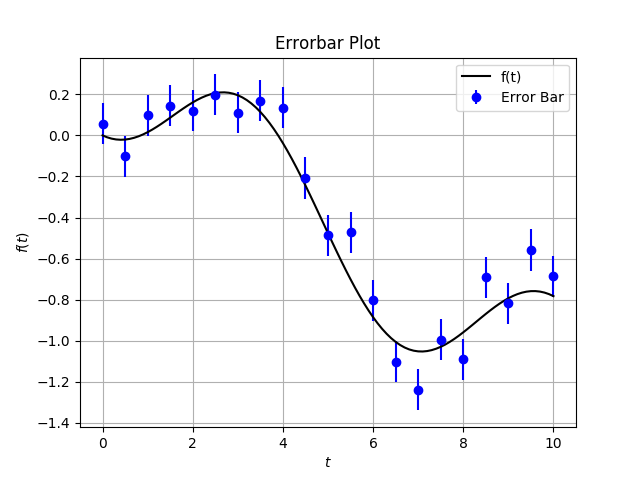
\includegraphics[scale=0.7]{Fig 1.png}
            \caption{$x(t)$ for $a=0.5$ and $\omega=1.5$}
            \label{fig:Fig1}
        \end{figure}

        If we use a smaller decay of $a=0.05$, then we get:
        \begin{figure}[H]
            \centering
            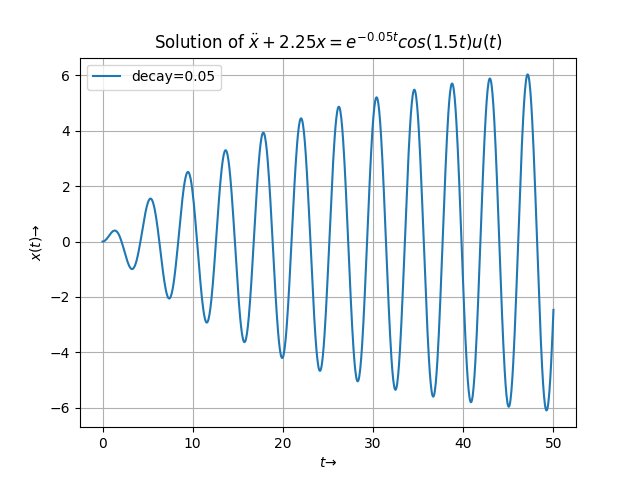
\includegraphics[scale=0.7]{Fig 2.png}
            \caption{$x(t)$ for $a=0.05$ and $\omega=1.5$}
            \label{fig:Fig2}
        \end{figure}

    \subsection{Response for different frequencies}
        Modeling the system as a LTI system and computing the response for various frequencies, we get:
        \begin{figure}[H]
            \centering
            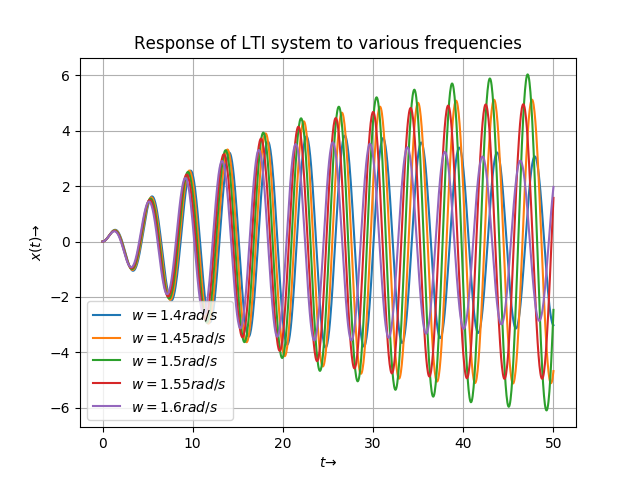
\includegraphics[scale=0.7]{Fig 3.png}
            \caption{$x(t)$ for $a=0.05$ and varying $\omega$}
            \label{fig:Fig3}
        \end{figure}

        From the given equation, we can see that the natural response of the system has the frequency $\omega= 1.5\ rad/s$.
        Thus, as expected, the maximum amplitude of oscillation is obtained when the frequency of $f(t)$ is $1.5\ rad/s$, as a case of resonance.
\section{Coupled Spring Problem}
    The coupled equations we are interested in solving are:
    \begin{gather*}
        \ddot{x} + (x-y) = 0\\
        \ddot{y} + 2(y-x) = 0
    \end{gather*}

    Substituting for $y$ from the $1^{\text{st}}$ equation, into the $2^{\text{nd}}$, we get a $4^{\text{th}}$ order differential equation in $x$:
    \begin{equation*}
        \ddddot{x} + 3\ddot{x} = 0
    \end{equation*}

    Given the ICs $x(0)=1$ and $\dot{x}(0)=y(0)=\dot{y}(0)=0$, we can write the above differential equation in the Laplace domain as:
    \begin{gather*}
        s^4\mathcal{X}(s)-s^3 + 3(s^2\mathcal{X}(s)-s)=0\\
        \implies \mathcal{X}(s) = \frac{s^2+3}{s^3+3s}\\
        \implies \mathcal{Y}(s) = \frac{2}{s^3+3s}
    \end{gather*}

    Solving for $x(t)$ and $y(t)$ is now very simple - use \texttt{scipy.signal.impulse} with the above $\mathcal{X}(s)$ and $\mathcal{Y}(s)$. We get the following graph for $x(t)$ and $y(t)$.
    \begin{figure}[H]
        \centering
        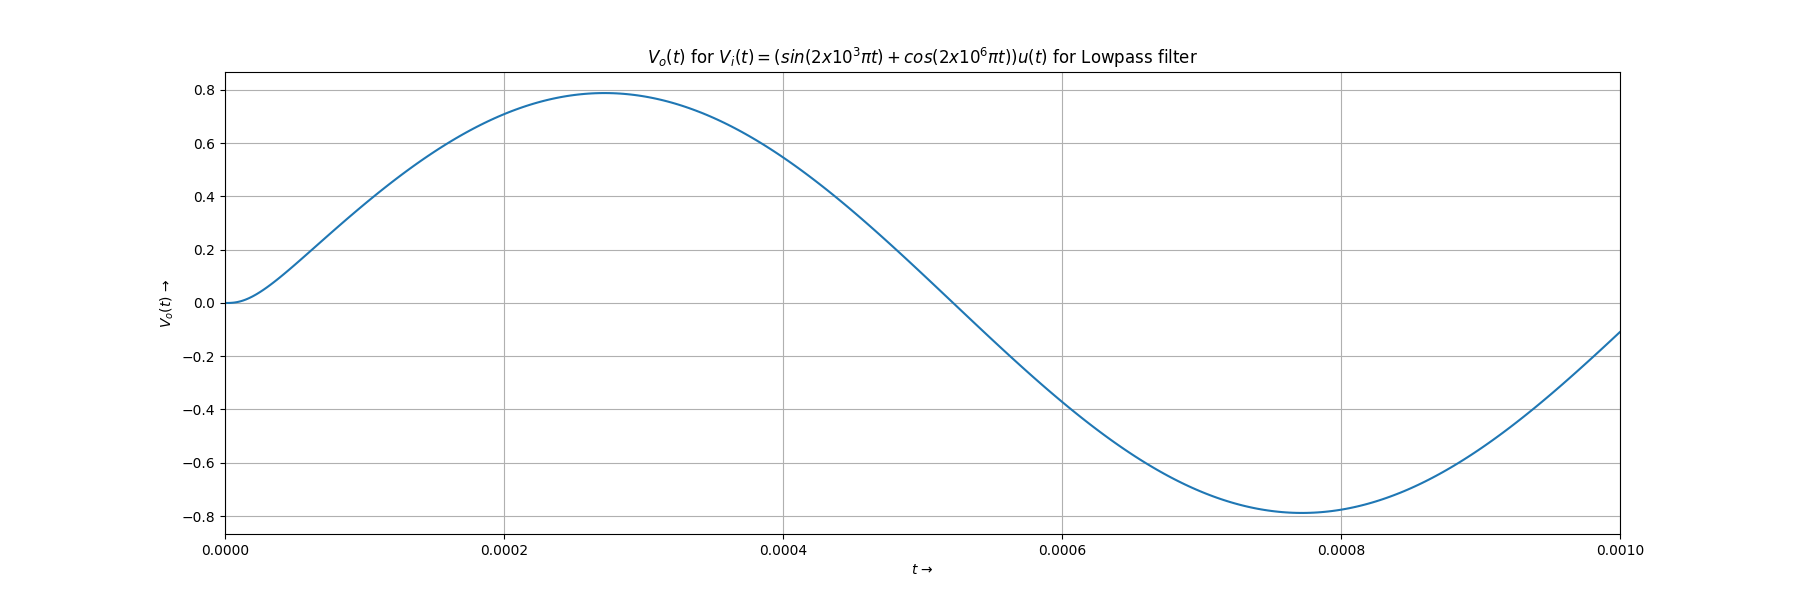
\includegraphics[scale=0.7]{Fig 4.png}
        \caption{$x(t)$ and $y(t)$ for the coupled spring problem}
        \label{fig:Fig4}
    \end{figure}

    We can see that $x(t)$ and $y(t)$ are sinusoids of the same frequency, but of different phase and magnitude.
\section{Two-port Network}
    The transfer function of the given two-port network can be written as:
    \begin{equation*}
        \frac{V_o(s)}{V_i(s)} = \mathcal{H}(s) = \frac{10^6}{s^2+100s+10^6}
    \end{equation*}

    The Bode magnitude and phase plots can be found using the method \texttt{scipy.signal.bode()}. The plots are shown below:
    \begin{figure}[H]
        \centering
        \setlength\tabcolsep{2pt}
        \begin{tabular}{cc}
            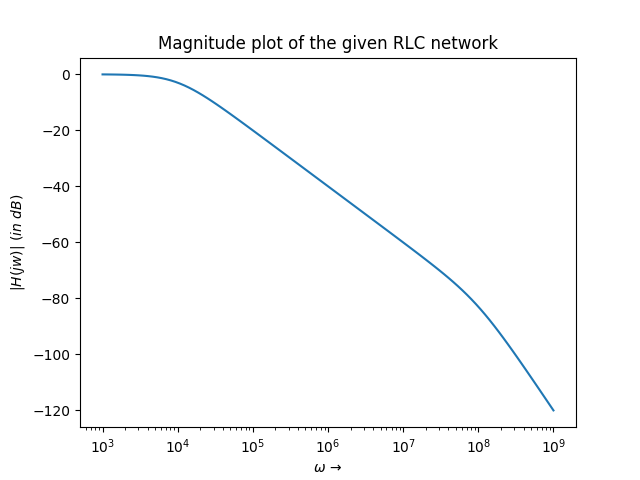
\includegraphics[scale=0.5]{Fig 5(a).png} &
            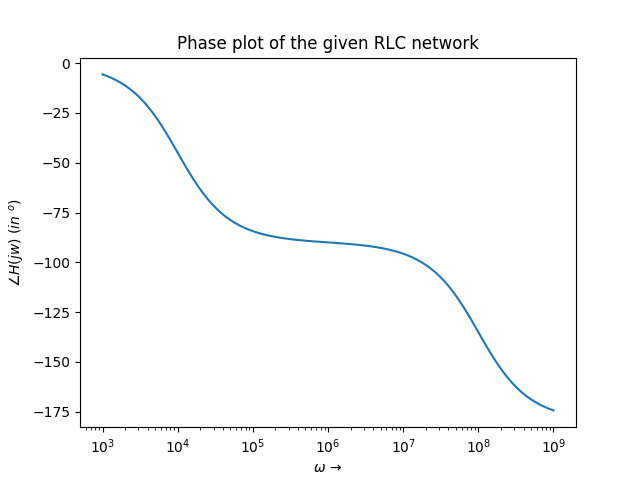
\includegraphics[scale=0.5]{Fig 5(b).png}\\
        \end{tabular}
        \caption{Bode Plots of the RLC Network's Transfer function}
    \end{figure}

    Now, when the input to the network, $v_i(t)$ is $(cos(10^3t)-cos(10^6t))u(t)$, the output is given by:
    \begin{equation*}
        V_o(s) = V_i(s)\mathcal{H}(s)
    \end{equation*}

    Since we have already found out $\mathcal{H}(s)$ and $V_i(s)$ can be easily found by using a lookup table (or by substituting $a=0$ in the equations used before), finding $v_o(t)$ is a simple task, thanks to \texttt{scipy.signal.lsim}. Plotting the obtained $v_o(t)$, we get:
    \begin{figure}[H]
        \centering
        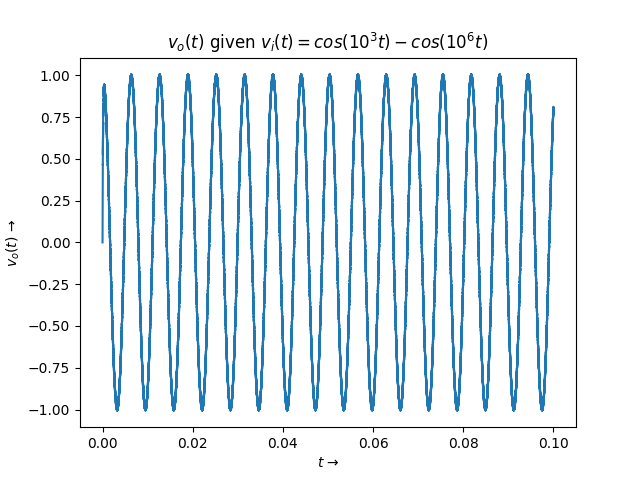
\includegraphics[scale=0.7]{Fig 6(a).png}
        \caption{$v_o(t)$ of the RLC network, when $v_i(t) = (cos(10^3t)-cos(10^6t))u(t)$}
        \label{fig:Fig6a}
    \end{figure}

    We can see it to be varying as a sinusoid of frequency approximately 160 Hz, which is expected, as the RLC network acts as a low pass filter - it allows low frequencies to pass through unchanged, while damping high frequencies to huge extent. We can see this in the graph. If we zoom in Figure (\ref{fig:Fig6a}), we can see the high frequency signal:
    \begin{figure}[H]
        \centering
        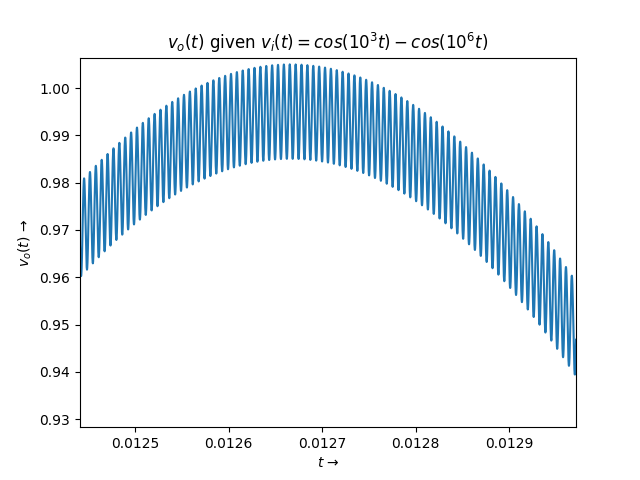
\includegraphics[scale=0.7]{Fig 6(c).png}
        \caption{High frequency signal in the output}
        \label{fig:Fig6c}
    \end{figure}

    We observe that the peak-to-peak amplitude of this high frequency variation is very less, approximately 0.02 V, compared to the initial 2 V. This is expected as we get a gain of -40dB at $\omega=10^6\ rad/sec$ from the bode plot, which corresponds to gain factor of 0.01.

    Another peculiarity of Figure (\ref{fig:Fig6a}) is the initial variation. When zoomed in, for $0<t<30\ us$, we get:
    \begin{figure}[H]
        \centering
        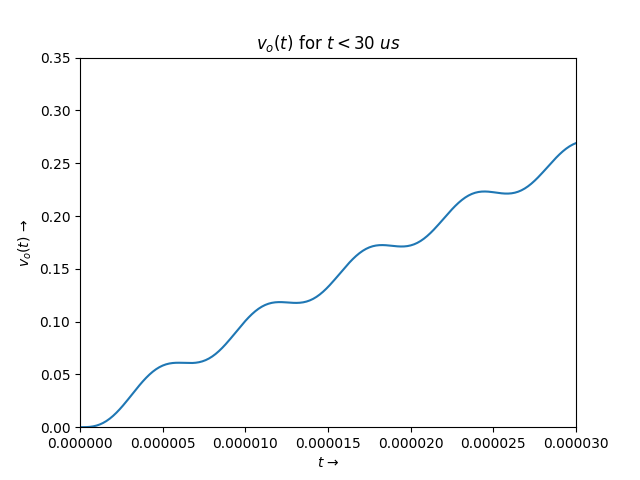
\includegraphics[scale=0.7]{Fig 6(b).png}
        \caption{Initial transients}
        \label{fig:Fig6b}
    \end{figure}

    This is due to application of the step input, i.e., the input is suddenly turned on at $t=0$.
\section{Conclusion}
To conclude, we analysed the solution of various continuous time LTI systems using Laplace transforms with help of \texttt{scipy.signal} toolbox.
\end{document}
